\documentclass[letterpaper]{physor2024}

%%% Packages Required by Class (already included)
% fancyhdr
% lastpage
% titling
% titlesec
% ragged2e
% enumitem
% amsmath
% graphicx
% geometry
% newtxtext
% newtxmath
% hyperref
% cleveref
% caption
% authblk
% apptools
% appendix
% ifpdf
% epstopdf

%%% Some other useful packages
% \usepackage{tikz}
% \usepackage{color}
% \usepackage{subcaption}
% \usepackage{algcompatible}
% \usepackage{bm}
% \usepackage{array}

% GLOSSARIES
\usepackage[acronym,nomain,nonumberlist,nogroupskip,nopostdot]{glossaries} % for glossary of acronyms
\setacronymstyle{long-short}
\loadglsentries{glossary}
\makeglossaries
% \renewcommand*{\glstextformat}[1]{\textcolor{black}{#1}} % make glossary color black

% % This file contains custom commands that Lewis uses frequently in LaTeX documents

\usepackage{subcaption}
\usepackage{hyperref}
\hypersetup{colorlinks,allcolors=black}
% % for more https://tex.stackexchange.com/questions/88400/hyperref-changing-the-linkcolor-locally-in-the-toc

% custom equation commands
\newcommand{\QOR}{\qquad \text{OR} \qquad}
\newcommand{\QAND}{\qquad \text{AND} \qquad}
\newcommand{\QTHUS}{\qquad \text{THUS} \qquad}
\newcommand{\QWITH}{\qquad \text{WITH} \qquad}
\newcommand{\QFOR}{\qquad \text{FOR} \qquad}
\newcommand{\QSO}{\qquad \text{SO} \qquad}
\newcommand{\QWHERE}{\qquad \text{WHERE} \qquad}
\newcommand{\QWHEN}{\qquad \text{WHEN} \qquad}
\newcommand{\LINE}{\par\noindent\rule{\textwidth}{0.4pt}\par}
\newcommand{\toinf}{\rightarrow\infty}
\newcommand{\tozero}{\rightarrow0}
\newcommand{\qeq}{\overset{?}{=}}
\newcommand{\ceq}{\overset{\checkmark}{=}}
\newcommand{\Poi}{\text{Poisson}}
\newcommand{\keff}{$k_{e\!f\!f}$}
\newcommand{\kinf}{$k_{\!i\!n\!f}$}
\renewcommand{\epsilon}{\varepsilon} % squiggly epsilon

\def\brac#1{\{#1\}}
\def\Brac#1{\big\{#1\big\}}
\def\BRAC#1{\bigg\{#1\bigg\}}
\def\angbrac#1{\langle#1\rangle}
\def\Angbrac#1{\big\langle#1\big\rangle}
\def\ANGBRAC#1{\bigg\langle#1\bigg\rangle}
\usepackage{float}
\usepackage{multirow} % for special table
% % SI Units
\usepackage{siunitx}
\DeclareSIUnit\n{n}
\DeclareSIUnit\sp{sp}
% \title{OpenMC Depletion Analysis of a TRISO Fueled, Helium Cooled Microreactor}
\title{Exploring Effects of Homogenization on an OpenMC Depletion Analysis of a TRISO Fueled, Helium Cooled Microreactor}

\addAuthor[ligross@wisc.edu]{Lewis I. Gross}{1}
\addAuthor{Patrick Shriwise}{2,1}
\addAuthor{Benjamin Lindley}{1}
\addAuthor{Paul P.~H. Wilson}{1}

%%% Affiliations (from authblk)
%%% \addAffiliation{affiliationNumber}{Name of Institute, City, State/Country}
\addAffiliation{1}{University of Wisconsin - Madison, Madison, Wisconsin}
\addAffiliation{2}{Argonne National Laboratory}

\Abstract{OpenMC is a state-of-the art, open-source Monte Carlo transport code. This work used OpenMC for depletion analysis of an infinite, unit cell model of the Virtual Test Bed gas-cooled microreactor. This microreactor is prismatic, TRISO-fueled, and helium gas cooled. Since the gas-cooled microreactor is intended for load-following, depletion analyses were conducted for 100\%, 50\%, and 10\% of the rated power (225 kW$_{th}$) both for fully explicit and partially explicit TRISO representation, along with a volume-homogenized comparison. The time steps selected ensure the same total burnup accrues at each step between the varying power levels. This study quantified the effects of homogenization on the $k$-eigenvalue to understand to what degree of explicit representation will be necessary for a full-core model. The system eigenvalue, \kinf, was computed as a function of burnup for each representation along with the pcm difference between each case with two-sigma error bars. Xenon-135 number density, which is a key factor explaining the observed \kinf~trends, are included. Due to the near identical results between fully explicit and kernel only TRISO representation, a full core model should use the kernel only representation to save memory while retaining sufficient accuracy.}

% The isotopics after one year of operation at steady-state were compared at each power for both homogenized and explicitly represented TRISO.

%%% List up to 5 keywords separated by a comma
\keywords{OpenMC, TRISO, depletion, microreactor, gas-cooled}

%%% Provide a short title for the header on odd pages
\shortTitle{Depletion of a TRISO Fueled, Gas-Cooled Microreactor }

%%% Provide a short author listing for the header on even pages
\authorHead{Gross and Wilson}

%%% If LaTeX reports the line number of an error at \begin{document} it
%%%   is most likely due to an error in one of the commands above
\begin{document}

\section{INTRODUCTION}\label{sec:intro}
For advanced reactors, especially those early in the design stage, sufficient \gls{ms} are required to ensure the success of the design concept. Before any system can be built, modelers must prove systems perform safely. The \gls{vtb} \cite{vtb2023} is a repository of reactor models used for research and demonstration of current tools in the nuclear industry as a part of the \gls{neams} initiative. Various types of reactors are available on the \gls{vtb}. Microreactors are one viable class of next generation systems with ongoing modeling efforts using \gls{neams} tools \cite{Stauff-preliminary-applications-2021, Stauff-applications-2022, Abdelhameed-ANS-2022}. One key advantage of microreactors is the ability to supply power to lower demand areas that may not be able to consume power on the order of a GW reactor or to areas needing temporary power, e.g.~natural disaster relief efforts. While microreactors can be diverse in fuel, coolant, and general design, there is interest in combining \gls{htgr} and microreactor technologies. \glspl{htgr} have the benefits of higher electricity conversion efficiency which synergizes with the higher melting temperature of \gls{triso} fuel. Adding these benefits to a microreactor brings many attractive features together.

Previous work on the \gls{vtb} \gls{gcmr} includes analysis of the system for a two day load-following transient \cite{Abdelhameed-ANS-2022}. This work coupled Griffin, BISON, and SAM using the \gls{moose} framework. Griffin computed a solution to the neutron transport equation using a deterministic method, specifically the discrete ordinates and discontinuous finite element methods with coarse mesh finite difference acceleration. BISON is a fuel performance code that computed heat conduction in the solid parts of the system. SAM is a systems analysis code that computed heat transfer in the coolant channels.

Due to the smaller size of microreactors, it is conceivable to move the reactor at some point during operation, e.g. if the system was only needed temporarily or if power is needed elsewhere, or after shutdown but before refueling. In this case, for shielding and criticality safety reasons, the state of the core must be fully understood. If a system has been running on the order of months, the core composition has certainly changed from the initial loading due to the effects of depletion. Since Abdelhameed et al.~only modeled 48 hours, depletion was not considered. Any analysis occurring far enough into an operation cycle requires a burnup simulation to know the state of isotopics in the core, whether computing an accident source term or shielding requirements for transporting the reactor after a shutdown.

A few depletion studies of other microreactor concepts exist, though this work adds the first depletion analysis to the \gls{vtb} \gls{gcmr}. A study of the gas-cooled, Japanese \gls{httr} computed criticality and burnup using various cross section representations with SCALE6 and MCNP5/X \cite{chiang-gcmr}. Another study looked at burnup for Westinghouse's eVinci \gls{hpmr}, finding that it could operate for at least 10 years without refueling, despite making more sense as a nuclear battery over a centralized power source \cite{Hernandez-hpmr}.

While previous work for the \gls{vtb} \gls{gcmr} used Griffin for neutron transport, this work chose OpenMC as an alternative to Griffin for a few reasons. First, OpenMC is an \gls{oss}. For this study, as well as others wishing to verify any OpenMC simulation, the code is freely available to use. As a Monte Carlo code, there are advantages over a deterministic code, like Griffin, for depletion analysis. The microscopic cross sections  are more accurate in continuous energy format when modeling the resonance region, as opposed to representing them with multi-group cross sections. There's also no need to do smaller studies to compute fine or coarse-group cross sections to produce diffusion coefficients with transport corrections for leakage, which is stronger in microreactors. OpenMC computes reaction rates--or optionally flux--directly from continuous energy cross sections as an input to depletion.

The rest of this paper will be organized as follows. \cref{sec:depletion} will provide some background theory on depletion. \cref{sec:openmc_model}  will detail the \gls{vtb} \gls{gcmr} and its components, explaining the OpenMC model and the depletion schemes. \cref{sec:results} will present results for the system. \cref{sec:conclusions} will interpret those results and discuss the plans forward for more \gls{ms}.

\section{DEPLETION THEORY}\label{sec:depletion}
Once any reactor starts running, the composition of isotopes will change over time. Nuclides exposed to neutron flux will transmute into radioisotopes that have various modes of decay, creating new isotopes that did not exist at the start of operation, as well as decaying into other isotopes already in the system. The rate at which isotopes transmute and decay into each other depends on the transport solution via the reaction rates, which depend directly on the neutron flux. This relationship causes the coupling between transport and depletion to behave non-linearly \cite{romano-depletion-2021}.

Certain isotopes have more influence on the system than others. For example, xenon-135 has an extremely high neutron absorption cross section, to the point that it influences the positioning of the control elements. Xenon-135 is important in load-following contexts, in which the power changes once or twice per day, as its concentration increases when power decreases, and it is burned off when power increases again. This matters more in load-following mode because the xenon-135 half-life is on the order of 9 hours \cite{d-and-h}. For context, the load following schedule in Abdelhameed et al. has high power for 12 hours, low power for 7 hours, and 2.5 hour ramps between, inspired from the NEA OECD report on load-following \cite{Abdelhameed-ANS-2022,nea-oecd-LF}.

To model burnup, transmutation and decay cross sections of the isotopes are combined with the computed flux to determine production and destruction rates for each isotope. These formulate a system of differential equations for the nuclide densities. For isotope $i$ with number density $N_{i}(t)$, the Bateman or burnup equations describe the time dependent isotopic composition, given by
\vspace*{-0.1cm}
\begin{multline} \label{eq:batemen}
    \frac{dN_{i}}{dt} =
    \sum_{j} \bigg[\int_{0}^{\infty} \sigma_{j\rightarrow{i}}(E,t)\phi(E,t)dE + \lambda_{j\rightarrow{i}}\bigg]N_{j}(t) \\
    -\bigg[\int_{0}^{\infty} \sigma_{i}(E,t)\phi(E,t)dE
    +\sum_{j}\lambda_{i\rightarrow{j}}\bigg] N_{i}(t),
\end{multline}

\noindent where $\sigma_{j\rightarrow{i}}(E,t)$ is the transmutation cross section of isotope $j$ that produces isotope $i$ at energy $E$ at time $t$, and $\lambda_{j\rightarrow{i}}$ are the decay constants for decay modes in nuclide $j$ that produce nuclide $i$. The system of equations for isotopes $i\in[1,n]$ can be expressed in matrix notation using the nuclide vector $\mathbf{n}\in\mathbb{R}^{n}$
\begin{equation} \label{eq:burnup matrix odes}
    \frac{d\textbf{n}}{dt} =
    \textbf{A}(\textbf{n},t) \textbf{n}
    \QWITH
    \textbf{n}(0) = \textbf{n}_{0},
\end{equation}

\noindent where $\textbf{A}\in\mathbb{R}^{n\times n}$ is the burnup matrix. Since the transport equation depends on number density and $\textbf{A}$ depends on the solution to the transport equation, $\textbf{A}$ then also depends on number density. Because ``the timescale over which material compositions change is sufficiently long ... the transport equation can be solved as a steady-state equation" \cite{romano-depletion-2021}. Taking the burnup equations as quasi steady-state allows the earlier non-separable equation to be solved via separation solution
\begin{equation} \label{eq:separable burnup matrix odes}
    \frac{d\textbf{n}}{dt} =
    \textbf{A}(\textbf{n}) \textbf{n}
    \QWITH
    \textbf{n}(0) = \textbf{n}_{0},
\end{equation}

\noindent The solution to which is
\begin{equation} \label{eq:separation solution}
     \textbf{n}(t) = e^{\textbf{A}t} \textbf{n}_{0}
\end{equation}

\noindent Solving \cref{eq:separable burnup matrix odes} numerically involves two separate components \cite{romano-depletion-2021}:
\begin{enumerate}
    \item Using a numerical method to integrate the matrix $\textbf{A}$ in \cref{eq:separable burnup matrix odes} forward in time. This usually involves taking one or more matrix exponential.
    \item Evaluating the matrix exponential $\exp(\textbf{A}t)$ or the action of the matrix exponential on a vector of nuclide concentrations.
\end{enumerate}

There are various methods for time integration. Predictor-Corrector methods are commonly used for time integration in burnup contexts. In this study, the second order \gls{cecm} is chosen, which is implemented by OpenMC, based on work comparing various integration schemes for depletion \cite{isotalo_comparison_2015}. Since the method is second order, it requires two transport solves per depletion time step: one for the prediction and one for the correction. Using appropriate time steps for the quasi static assumption of burnup is also important. Namely, using smaller time steps when nuclide concentrations are expected to be changing more rapidly and larger time steps when nuclide concentrations are expected to be changing more slowly. \textbf{add something about our time step choice?}

\section{OPENMC MODEL}\label{sec:openmc_model}
This section will describe the \gls{gcmr} system and OpenMC model, which has two phases. In the first phase, OpenMC generates geometry and material definitions. In the second, OpenMC loads these definitions, defines depletion settings, and launches the alternating transport, depletion, and nuclide updates.

\subsection{System Description}\label{sec:system}
\vspace*{-0.05cm}
 \cref{fig:vtb_gcmr} shows a diagram of the \gls{gcmr}. Graphite is the structural material holding the cylindrical compacts arranged in a hexagonal lattice. \cref{tab:dimensions} shows various system parameters. The fuel compacts contain \gls{triso} spheres packed into graphite. The moderator uses YH$_{2}$ with a thin Cr coating encased in a FeCrAl envelope; the coating is between the YH$_{2}$ and the envelope. The poison compacts contain burnable B$_{4}$C spheres packed into graphite. The coolant is helium. The upper and lower reflectors are BeO. Since the goal of this work is to determine excess reactivity, this model rests a B$_{4}$C control rod in the upper reflector; it is not inserted into the active core region, which instead is filled with non-circulating helium \cite{Abdelhameed-ANS-2022}. A cosine heating distribution was used to approximate temperature: inlet $T=873.15$ K, outlet $T=1133.65$ K. The lower reflector was set to the inlet temperature and the upper reflector was set to the outlet temperature.
\vspace*{-0.2cm}
 \begin{figure}[h]
    \centering
    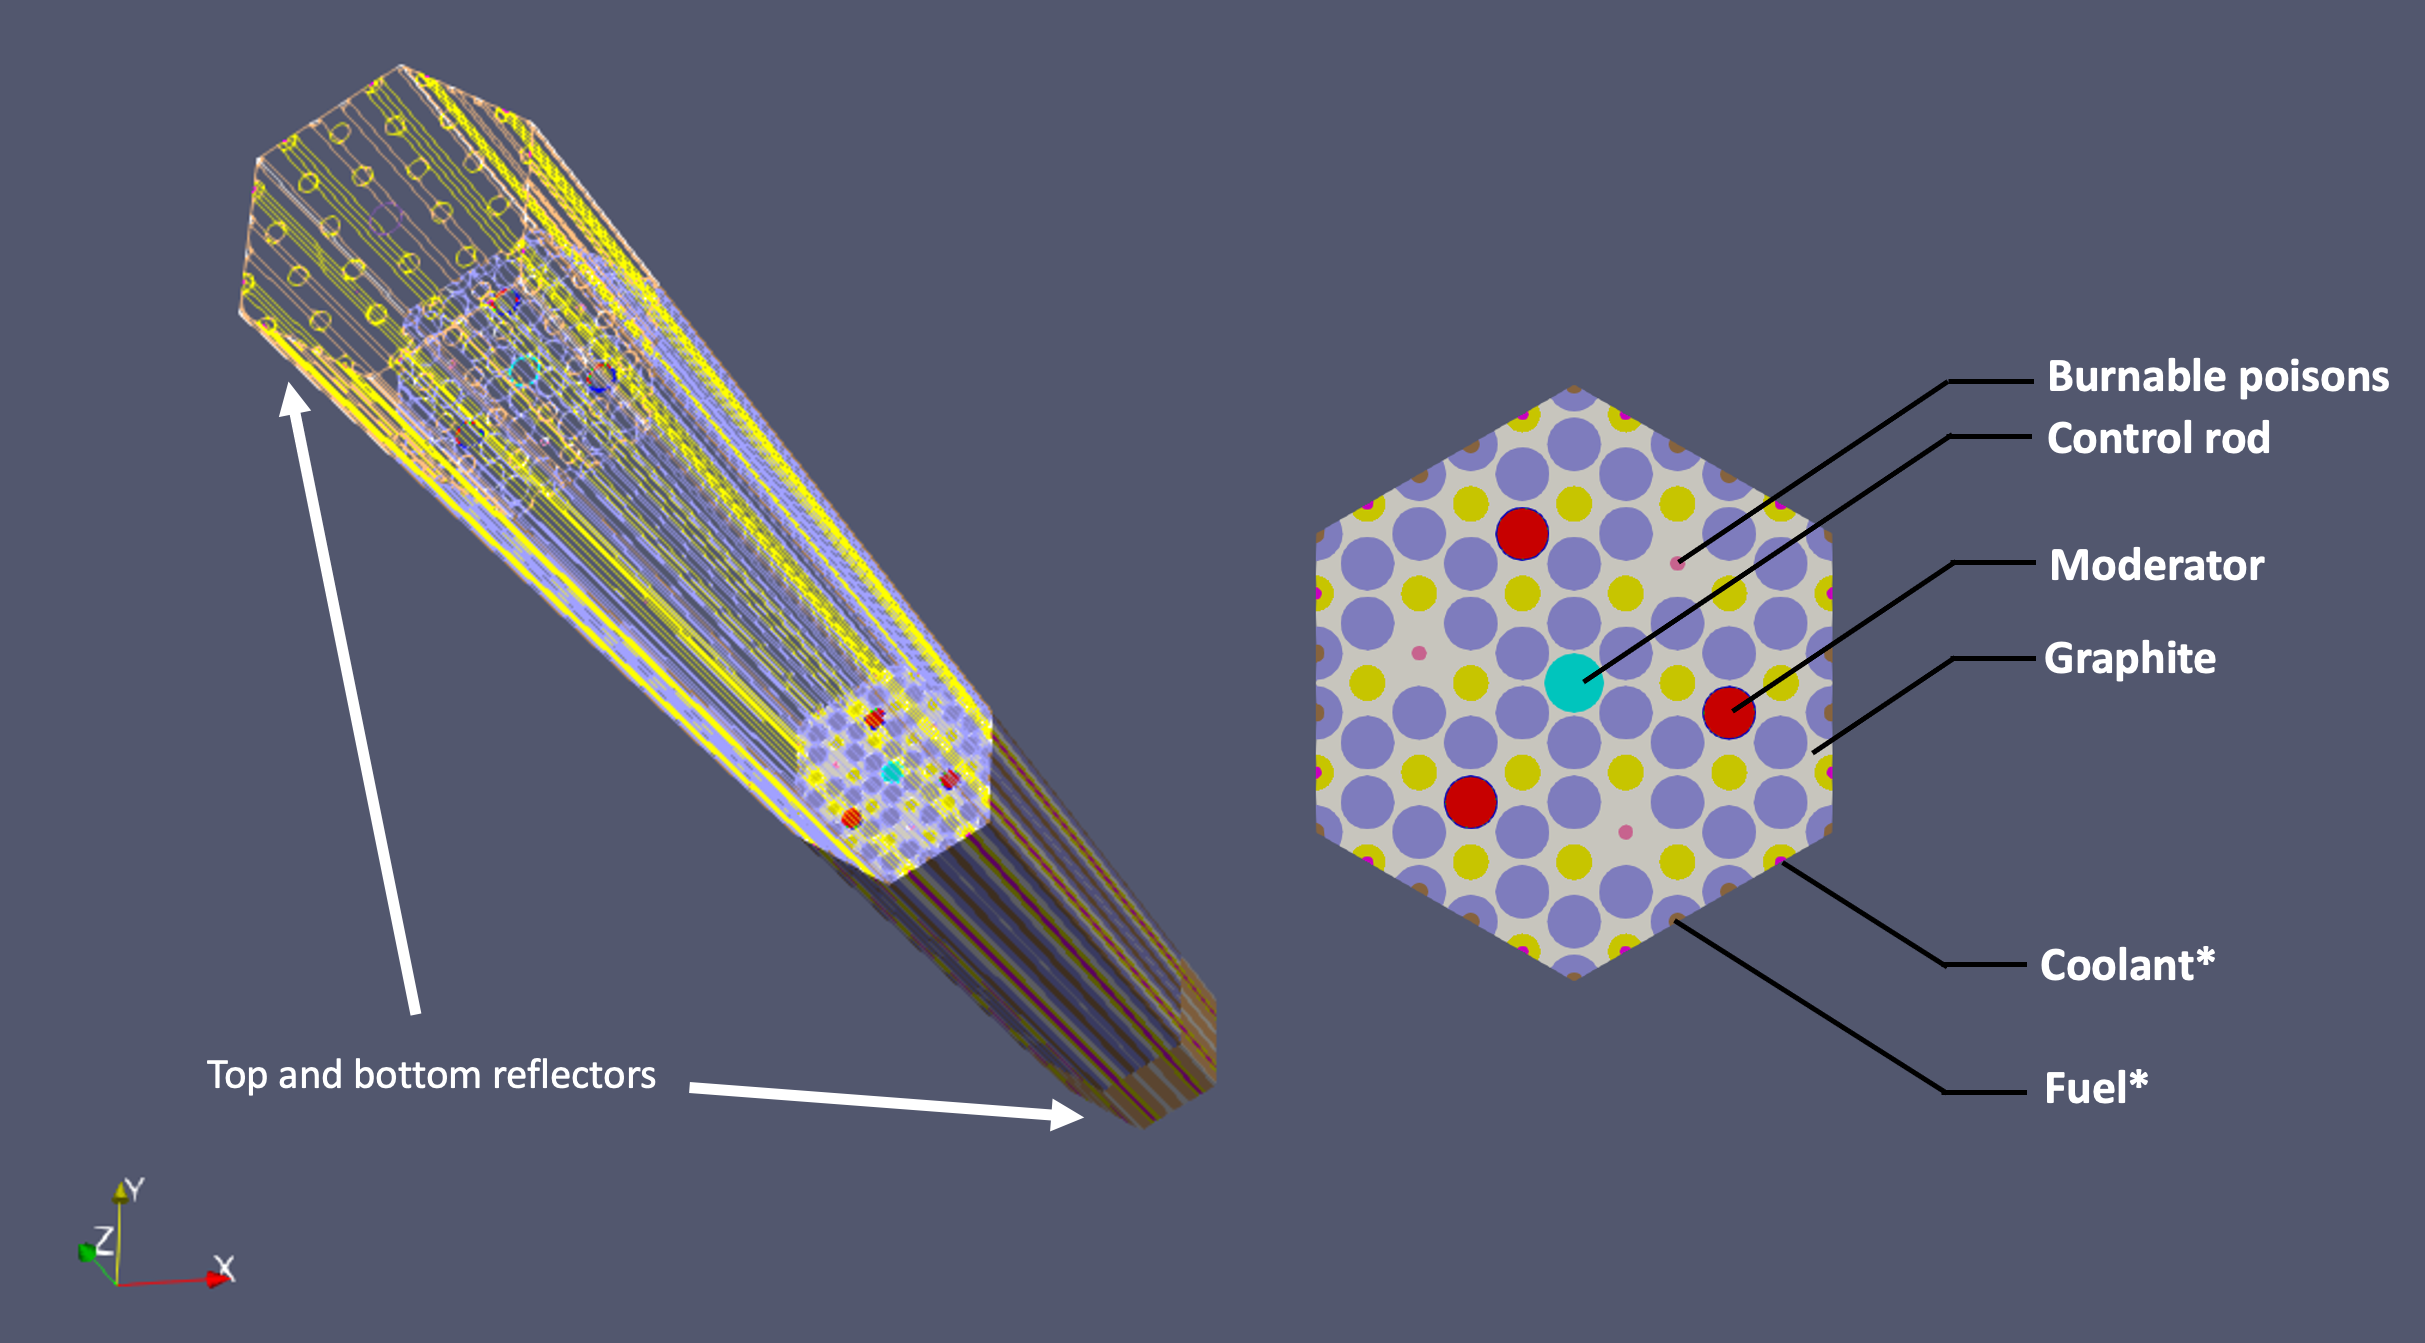
\includegraphics[width=0.6\linewidth]{figures/vtb_gcmr_diagram.jpg}
    \caption{The above visualization shows the \gls{vtb} \gls{gcmr} unit cell: both a cross section of the fuel region and a 3D rendering of the fuel and reflectors \cite{Stauff-applications-2022}.}
    \label{fig:vtb_gcmr}
\end{figure}
\vspace*{-0.5cm}
\begin{table}[h]
    \centering
    \caption{This table summarizes key dimensions (radii, thicknesses) of the compacts and parameters of the fuel and poison.}
    \begin{tabular}{|c|c|c|c|c|c|}
    \hline
    fuel radius & poison radius & moderator radius, Cr coating & control radius & coolant radius \\
    0.90 cm & 0.25 cm   & 0.843 cm, 0.007 cm & 0.99 cm    & 0.60 cm  \\
    \hline
    FeCrAl thickness & pin pitch & fuel packing fraction & poison packing fraction & enrichment \\
    0.05 cm & 2.00 cm  & 0.4 -  & 0.25 - & 19.95\% \\
    \hline
    \end{tabular}
    \vspace{-0.5cm}
    \label{tab:dimensions}
\end{table}
\subsection{Model Definition}\label{sec:model_def}
With the goal of quantifying effects of homogenization, simulations with fully explicit and partially explicit \gls{triso} representations are included along with a fully homogenized fuel case. The partial representation, herein named ``kernel only," packed fuel kernels--maintaining the correct packing fraction of kernels--while homogenizing the various outer graphite-like and silicon carbide layers into the background graphite. The only differences between these models are the fuel representation, with all other compacts being defined exactly the same. The system is divided into axial layers to allow for spatial variation in depletion. While \cite{Abdelhameed-ANS-2022} chose two axial layers per reflector and 16 layers in the active region, due to memory constraints, all cases in this study used eight layers in the active region. The reflectors are 20 cm high and the core is 160 cm high. Within each layer, fuel compacts are depleted identically to their two sister compacts at the corresponding symmetry points (3-way symmetry), yielding 18 unique depletable fuel regions per layer. Additionally, to allow the B$_{4}$C to burn, poison compacts add a 19th depletable region per layer. \cref{fig:core_slice_sbs} shows a radial slice of the fuel portion of the reactor. \cref{fig:reflectors} shows a radial slice of each reflector region.

\begin{figure}[!h]
    \centering
    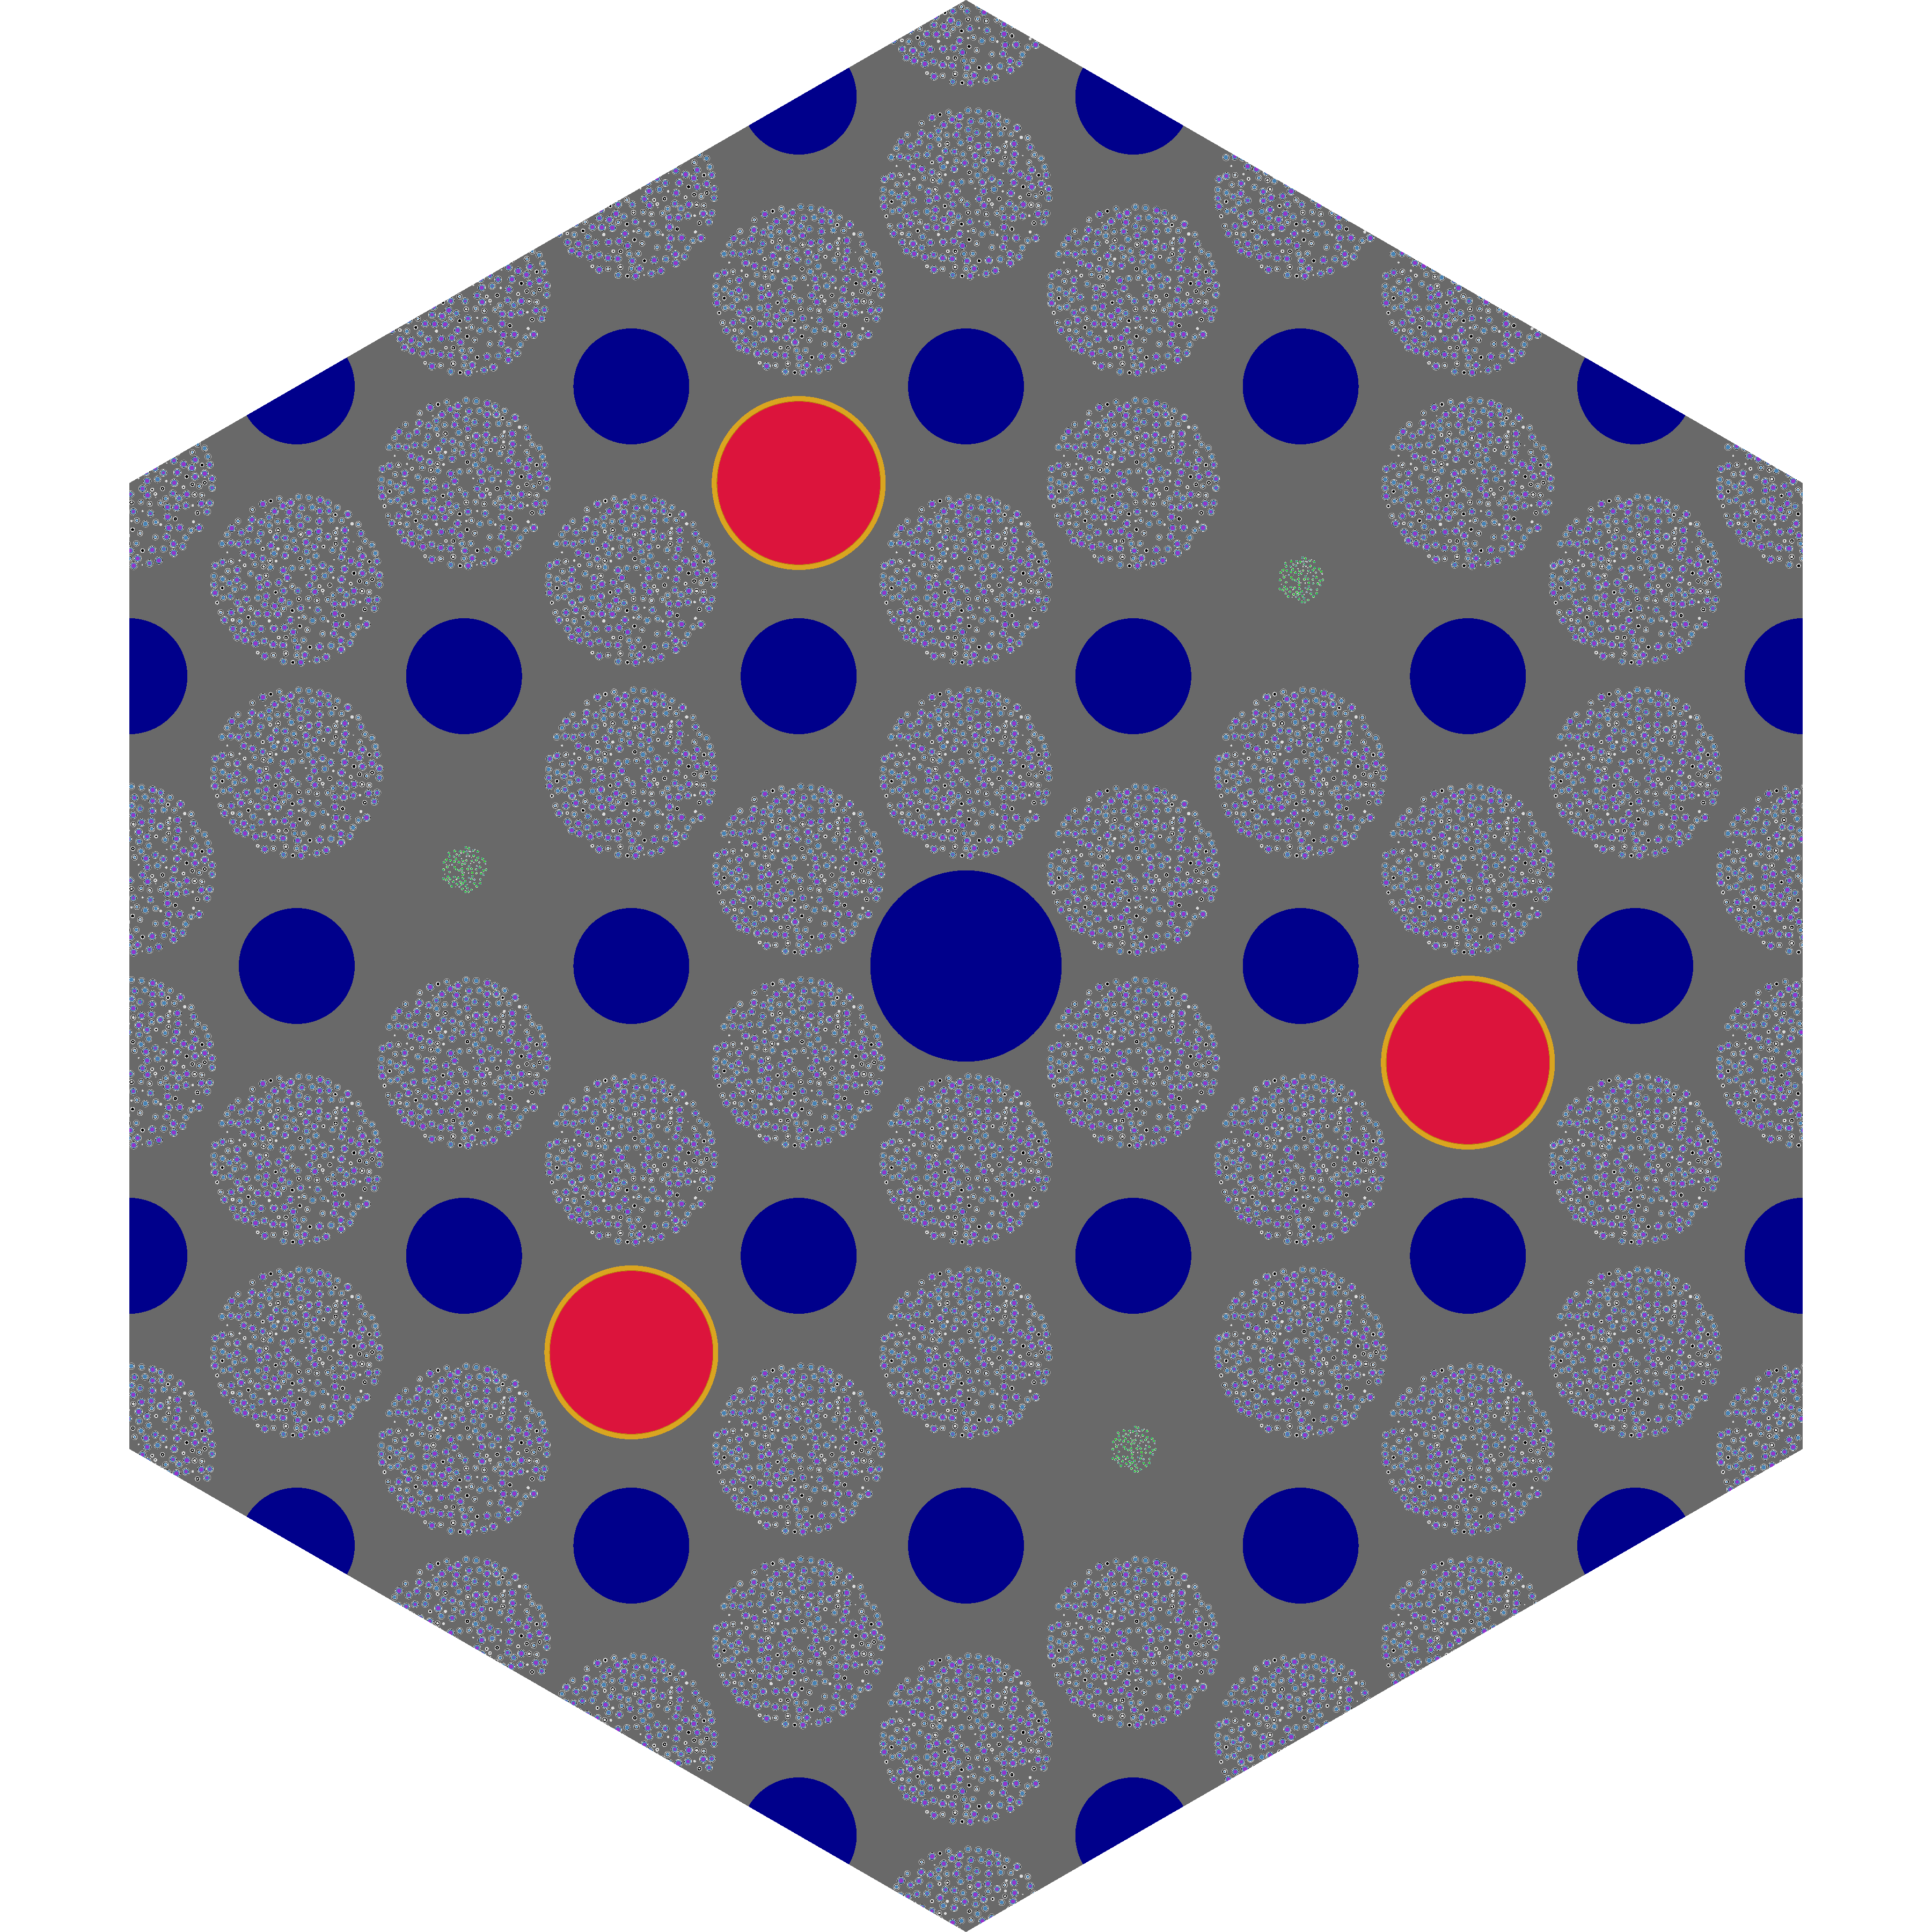
\includegraphics[width=0.375\linewidth]{figures/active_height.png}
    \label{fig:active_slice}
    \caption{This figure shows a radial slice of the active region. Gray corresponds to graphite in the matrix or pyrolitic carbon, dark blue corresponds to helium coolant, red corresponds to YH$_{2}$ moderator, gold corresponds to FeCrAl, green corresponds to the B$_{4}$C poison particles (packed at 25 percent in graphite), and purple corresponds to the fuel kernel in the \gls{triso} particles (packed at 40 percent in graphite).}
    \label{fig:core_slice_sbs}
\end{figure}
\begin{figure}[!h]
    \centering
    \begin{subfigure}{0.475\linewidth}
        \centering
        
\includegraphics[width=0.7\linewidth]{figures/lower_reflector.png}
        \caption{A slice of the lower reflector, colored by material.}
        \label{fig:lower_reflector_slice}
    \end{subfigure}
    \begin{subfigure}{0.475\linewidth}
        \centering
        
\includegraphics[width=0.7\linewidth]{figures/upper_reflector.png}
        \caption{A slice of the upper reflector, colored by material.}
        \label{fig:upper_reflector_slice}
    \end{subfigure}
    \caption{This figure shows a  radial slice of the lower reflector (left) and the upper reflector (right). The difference between the upper and lower reflectors is that the upper reflector has an extra compact for the B$_{4}$C control rod. Dark blue corresponds to helium coolant and light blue corresponds to BeO, while the B$_{4}$C control rod is shown in green.}
    \label{fig:reflectors}
    \vspace*{-0.4cm}
\end{figure}

\subsection{Depletion Simulation Definition}\label{sec:depl_sim}
With complete geometry and material definitions, the depletion simulation defines power history, time steps, and an integration scheme. OpenMC then alternates between transport and Batemen equation solves. The eigenvalue simulations used 25 inactive batches and 75 active batches with 10000 particles per batch. The cross sections used for transport are continuous energy from ENDF-B-VII.1. The chain file, an XML file used for depletion in OpenMC, contains transmutation and decay data necessary to compute the burnup matrix. This simulation used a chain based on the \gls{casl} project \cite{CASL-report} and is provided by OpenMC \cite{openmc-chains}. While the chain originates from a \gls{lwr} system, the similarity of the neutron spectrum, i.e. both thermal, makes this chain file a good choice, since $\phi(E)$ is one of the inputs when computing the burnup matrix. The \gls{casl} chain can be found on OpenMC's website, specifically the portion that provides data for users to download.

To account for the initial rapid build up of strong neutron absorbers, the first few time steps are shorter to increase those nuclides' accuracy. The time steps can be lengthened after the nuclides' initial transient behavior reaches a steady-state. For all full power cases, the time steps used: five one-day time steps, three five-day time steps, three fifteen-day time steps, and 25 60 day time steps. In order to keep the burnup the same at each step for all other powers, the half and tenth power cases use the same number of steps, with twice and ten times as long steps, respectively.

\section{RESULTS}\label{sec:results}
The main comparison to assess the necessity of explicit representation is \kinf~as a function of burnup. \cref{fig:kinf_full_explicit_results} shows \kinf~vs burnup with two-sigma error bars for the fully explicit case. \cref{fig:pcm_diffs} shows the difference in \gls{pcm} between each representation with propagated two-sigma error bars.

\begin{figure}[!h]
    \centering
    \begin{subfigure}{0.7\linewidth}
        \centering
        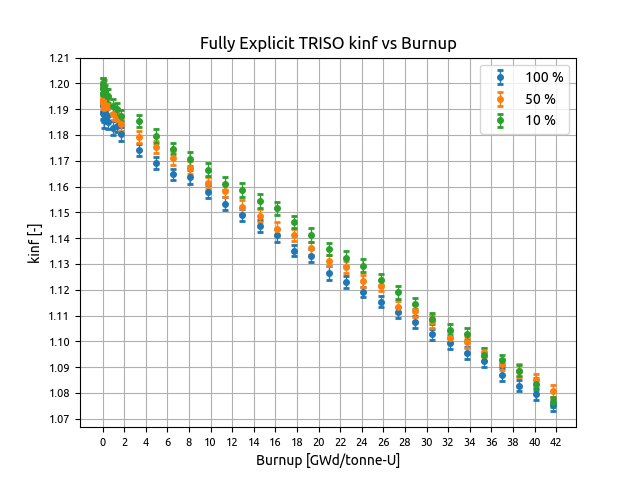
\includegraphics[width=\linewidth]{figures/expl_kinf_vs_bu.png}
    \end{subfigure}
    \caption{This figure shows \kinf versus burnup for the fully explicit case with two-sigma error bars up to $\sim$42 GWd/tonne-U. The legend shows that 100\% power is blue, 50\% power is orange, and 10\% power is green. }
    \label{fig:kinf_full_explicit_results}
\end{figure}

\begin{figure}[!h]
    \centering
    \begin{subfigure}{0.495\linewidth}
        \centering
        \includegraphics[width=\linewidth]{figures/explicit_minus_homog.png}
        \caption{Explicit minus homogenized}
    \end{subfigure}
    \begin{subfigure}{0.495\linewidth}
        \centering
        \includegraphics[width=\linewidth]{figures/kern_minus_homog.png}
        \caption{Kernel only minus homogenized}
    \end{subfigure}
    \begin{subfigure}{0.495\linewidth}
        \centering
        \includegraphics[width=\linewidth]{figures/explicit_minus_kern.png}
        \caption{Explicit minus kernel only}
    \end{subfigure}
    \caption{This figure shows the \gls{pcm} difference versus burnup with two-sigma error bars on \kinf for the pairs of each representation up to a burnup of $\sim$42 GWd/tonne-U. Each legend shows that 100\% power is blue, 50\% power is orange, and 10\% power is green.}
    \vspace*{-0.3cm}
    \label{fig:pcm_diffs}
\end{figure}

When homogenizing \gls{triso}, the differences in eigenvalue come from slowing down of neutrons, specifically which materials they interact with as they thermalize and attempt to cause new fissions. A fully explicit \gls{triso} has layers of pyrolitic carbon and silicon carbide surrounding the kernel. When \gls{triso} is fully homogenized, neutrons have less chance to thermalize before interacting with fuel atoms, and thus are more likely to be absorbed in a resonance. However, the slowing down of neutrons in background graphite is expected to be similar to slowing down in the non-fuel \gls{triso} shells, motivating the kernel only case. Despite the known inaccuracies of fully homogenized compacts, this work aims to quantify the actual \gls{pcm} difference in the eigenvalue for the \gls{gcmr} as a basis for what kind of representation must be included in a full core model. The initial and final eigenvalue will now be reported for each case.

\begin{itemize}
    \item explicit
    \begin{itemize}
        \item 100\% \kinf: $1.19995 \pm 0.00218 \xrightarrow{} 1.07539 \pm 0.00223$
        \item 50\% \kinf: $1.19995 \pm 0.00218 \xrightarrow{} 1.08086 \pm 0.00231$ \item 10\% \kinf:  $1.19995 \pm 0.00218 \xrightarrow{} 1.07661 \pm 0.00193$
    \end{itemize}
    \item kernel only
    \begin{itemize}
        \item 100\% \kinf: $1.20229 \pm 0.00262 \xrightarrow{} 1.07855 \pm 0.00247$
        \item 50\% \kinf: $1.20229 \pm 0.00262 \xrightarrow{} 1.08568 \pm 0.00235$
        \item 10 \% \kinf: $1.20229 \pm 0.00262 \xrightarrow{} 1.08328 \pm  0.00245$.
    \end{itemize}
    \item homogenized
    \begin{itemize}
        \item 100\% \kinf: $ 1.17285 \pm 0.00229 \xrightarrow{} 1.04950 \pm 0.00200 $
        \item (50\%) \kinf: $ 1.17285 \pm 0.00229 \xrightarrow{} 1.05397 \pm 0.00214 $
        \item (10\%) \kinf: $1.17285 \pm 0.00229 \xrightarrow{} 1.05101 \pm 0.00217$
    \end{itemize}
\end{itemize}

There are a few key features of the results. While only the explicit case was shown in \cref{fig:kinf_full_explicit_results}, all cases experience a similar trend where increasing power results in less excess reactivity, despite each depletion step using the same total burnup. The difference between the power levels diminish as higher burnups are achieved, to the point near the end of the simulation, over 34 GWd/tonne-U, all three power levels eigenvalues are more or less overlapping when considering a two-sigma confidence interval. In order to explain the trends, it will be useful to examine the xenon-135 atom densities for each case, shown in \cref{fig:xenons}.

\begin{figure}[!h]
    \centering
    \begin{subfigure}{0.495\linewidth}
        \centering
        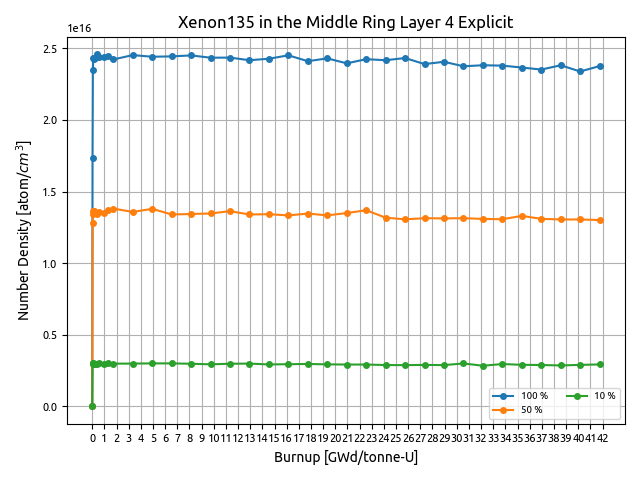
\includegraphics[width=\linewidth]{figures/expl_xe135.png}
    \end{subfigure}
    \begin{subfigure}{0.495\linewidth}
        \centering
        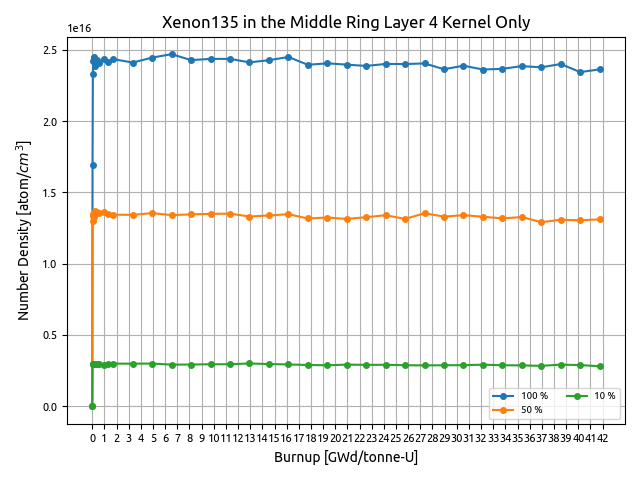
\includegraphics[width=\linewidth]{figures/kern_xe135.png}
    \end{subfigure}
    \begin{subfigure}{0.495\linewidth}
        \centering
        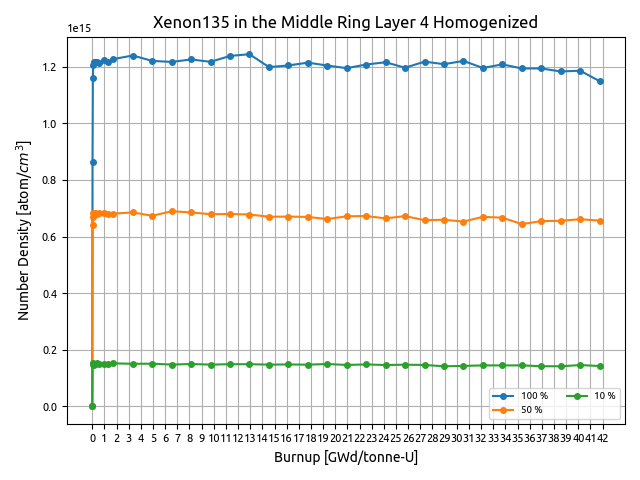
\includegraphics[width=\linewidth]{figures/homog_xe135.png}
    \end{subfigure}
    \caption{This figure shows the xenon-135 number density up to $\sim$42 GWd/tonne-U from a fuel compact in the middle layer in the innermost ring. Each representation's plot shows the three power levels computed.}
    \label{fig:xenons}
\end{figure}

In each case, xenon-135 concentration jumps to an equilibrium level quickly. The higher the power, the higher the equilibrium xenon concentration. More xenon means more competition with absorptions in fuel. This explains why the higher powers have less excess reactivity, since the xenon negative insertions are larger at higher power, despite the same total burnup (same percent atoms fissioned).

The most important take away can be seen from \cref{fig:pcm_diffs}. Overall, there's seemingly no trend with respect to burnup about the actual pcm difference, as most cases two-sigma confidence intervals are overlapping. The difference between fully explicit and homogenized ranges from about 200-300 \gls{pcm}. The difference between kernel only and homogenized ranges from about 230 - 330 \gls{pcm}. These two differences are near indistinguishable, meaning that the kernel only representation performs as well as the fully explicit modeling. Another interesting takeaway is that the pcm difference between fully explicit and kernel only ranges from -80-20 \gls{pcm} near one order of magnitude smaller. All of this evidence points to the conclusion that a kernel only representation will be sufficient for full core modeling.

\section{CONCLUSIONS}\label{sec:conclusions}
This paper simulated an infinite, unit cell model of the \gls{vtb} \gls{gcmr} using the OpenMC Monte Carlo code, adding the first depletion analysis for this reactor. Since the reactor is intended to load follow, it depleted the system at $100\%$, $50\%$ and $10\%$ power. The depletion simulations showed that the reactor still has excess reactivity to at least 42 GWd/tonne-U and likely could extend to upwards of 50 GWd/tonne-U. The comparisons between fully explicit and kernel only show that the kernel only representation is sufficient for this system, yielding nearly identical results. The kernel only representation alleviates memory consumption, which only will become more of a limiting factor for modeling a full core. While the homogenized case uses a much smaller fraction of the memory, the 200+ \gls{pcm} difference is too much to trust the results. An important next step will be to model depletion during repeated load following transients and to deplete in a critical configuration to verify the same conclusions.

Standalone depletion is a first step in understanding the \gls{gcmr}, but it is of interest to couple depletion into a multiphysics algorithm to aim for as high fidelity simulations as possible. Future multiphysics analyses will rely on Cardinal \cite{novak2022-cardinal}. The Cardinal simulation will couple OpenMC for neutron transport, \gls{moose}'s \gls{htm} for heat conduction, and \gls{thm} for 1-D thermal hydraulics. After verification of standalone simulations, it will be of interest to quantify the impact of depletion on high-fidelity multiphysics.

\section*{ACKNOWLEDGEMENTS}
The authors would like to thank the OpenMC development team for their guidance and assistance with software, as well as the Center for High Throughput Computing at the University of Wisconsin - Madison for their support in using the High Performance Cluster. The first author was supported in part by the US Nuclear Regulatory Commission's Graduate Fellowship Program administered by the University of Wisconsin-Madison.

% \printglossaries

\bibliographystyle{physor2024}
\bibliography{physor2024}

\end{document}